\begin{figure}[t]
\centering
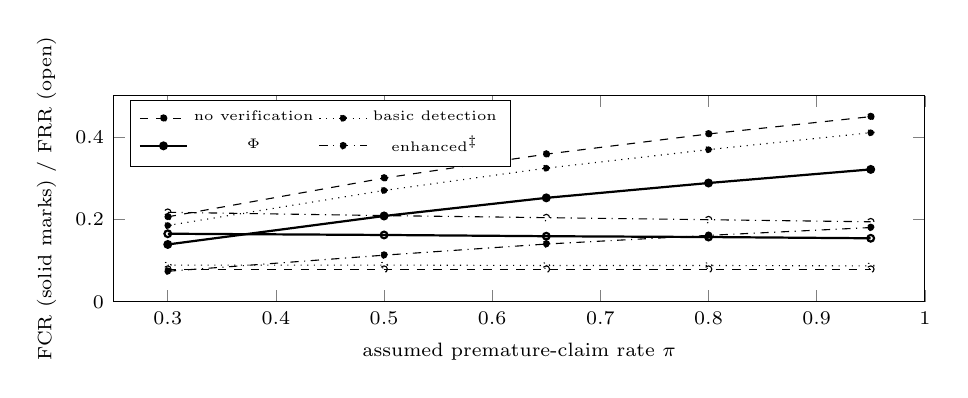
\begin{tikzpicture}
\begin{axis}[width=0.98\columnwidth, height=4.2cm, xlabel={assumed premature-claim rate $\pi$}, ylabel={FCR (solid marks) / FRR (open)},
  xmin=0.25, xmax=1.0, ymin=0, ymax=0.5, legend style={font=\tiny, at={(0.02,0.98)}, anchor=north west, legend columns=2},
  tick label style={font=\scriptsize}, label style={font=\scriptsize}]
\addplot[dashed, mark=*, mark size=1.2pt] coordinates {(0.3,0.206) (0.5,0.300) (0.65,0.358) (0.8,0.407) (0.95,0.449)};
\addlegendentry{no verification}
\addplot[dotted, mark=*, mark size=1.2pt] coordinates {(0.3,0.185) (0.5,0.270) (0.65,0.324) (0.8,0.369) (0.95,0.410)};
\addlegendentry{basic detection}
\addplot[thick, mark=*, mark size=1.2pt] coordinates {(0.3,0.139) (0.5,0.208) (0.65,0.252) (0.8,0.288) (0.95,0.321)};
\addlegendentry{$\Phi$}
\addplot[dashdotted, mark=*, mark size=1.2pt] coordinates {(0.3,0.074) (0.5,0.113) (0.65,0.140) (0.8,0.161) (0.95,0.180)};
\addlegendentry{enhanced$^{\ddagger}$}
\addplot[dashed, mark=o, mark size=1.2pt, forget plot] coordinates {(0.3,0.079) (0.5,0.079) (0.65,0.079) (0.8,0.079) (0.95,0.079)};
\addplot[dotted, mark=o, mark size=1.2pt, forget plot] coordinates {(0.3,0.089) (0.5,0.089) (0.65,0.088) (0.8,0.088) (0.95,0.087)};
\addplot[thick, mark=o, mark size=1.2pt, forget plot] coordinates {(0.3,0.165) (0.5,0.162) (0.65,0.159) (0.8,0.157) (0.95,0.154)};
\addplot[dashdotted, mark=o, mark size=1.2pt, forget plot] coordinates {(0.3,0.217) (0.5,0.209) (0.65,0.204) (0.8,0.199) (0.95,0.194)};
\end{axis}
\end{tikzpicture}
\caption{\textsc{Simulation-based (synthetic)} Study~H: mean FCR and FRR over 300 regenerated scenario sets per point as the assumed rate at which the planner claims completion of an unfinished task varies. Stricter verification lowers FCR at every rate and raises FRR; its FCR advantage grows with $\pi$. $^{\ddagger}$Not implemented.}
\label{fig:sim-sens}
\end{figure}
